\documentclass[xcolor=svgnames]{beamer}
\usepackage[utf8]{inputenc}
\usepackage[T1]{fontenc}
\usepackage{xcolor}
\usepackage{booktabs}
\usepackage{amsmath}
\usepackage{graphicx}
\usepackage{hyperref}
\usepackage{mhchem}
\usepackage{tikz} % For flowchart example
\usetikzlibrary{shapes, arrows, positioning}

\usetheme{Madrid}

% COLORS (As provided)
\definecolor{mqred}{RGB}{166, 25, 46}
\definecolor{mqdeepred}{RGB}{118, 35, 47}
\definecolor{mqgray}{RGB}{55, 58, 54}
\definecolor{mqlightgray}{RGB}{237, 235, 229}
\definecolor{mqmagenta}{RGB}{198, 0, 126}
\usecolortheme[named=mqred]{structure}
\setbeamercolor{title in head/foot}{bg=mqlightgray, fg=mqgray}
\setbeamercolor{author in head/foot}{bg=mqdeepred}
\setbeamercolor{page number in head/foot}{bg=mqdeepred, fg=mqlightgray}

% FOOTNOTE ARRANGEMENTS (As provided)
\makeatletter
\setbeamertemplate{footline}{
  \leavevmode%
  \hbox{%
  \begin{beamercolorbox}[wd=.5\paperwidth,ht=2.25ex,dp=1ex,center]{author in head/foot}%
    \usebeamerfont{author in head/foot}\insertshortauthor\expandafter\ifblank\expandafter{\beamer@shortinstitute}{}{~~(\insertshortinstitute)}
  \end{beamercolorbox}%
  \begin{beamercolorbox}[wd=.4\paperwidth,ht=2.25ex,dp=1ex,center]{title in head/foot}%
    \usebeamerfont{title in head/foot}\insertshorttitle
  \end{beamercolorbox}%
  \begin{beamercolorbox}[wd=.1\paperwidth,ht=2.25ex,dp=1ex,center]{page number in head/foot}%
    \usebeamerfont{page number in head/foot}\insertframenumber{} / \inserttotalframenumber
  \end{beamercolorbox}}%
  \vskip0pt%
}
\makeatother
\beamertemplatenavigationsymbolsempty

% TITLE, AUTHORS, INSTITUTE, DATE
\title[Org Chem: Designing Syntheses]{Lesson 3: Designing \& Communicating Syntheses}
\subtitle{Mastering Flowcharts (CHM\_M7\_SYNTH\_N1)}
\author[P. Haynes]{Mr Haynes} % Replace if needed
\institute[GHS]{Gosford High School}
\date{Module 7: Organic Chemistry}

\begin{document}

\begin{frame}
    \titlepage
\end{frame}

\begin{frame}{Outline}
    \tableofcontents
\end{frame}

\section{The Complete Picture}
\begin{frame}{Reviewing the Full Map}
    \frametitle{The Interconnected Network}
    Let's look at the full reaction map (Chord Diagram) incorporating all the reactions we've learned in this module.
    \vspace{1em}
    \begin{figure}
        % Replace with screenshot of the full, relevant chord diagram
        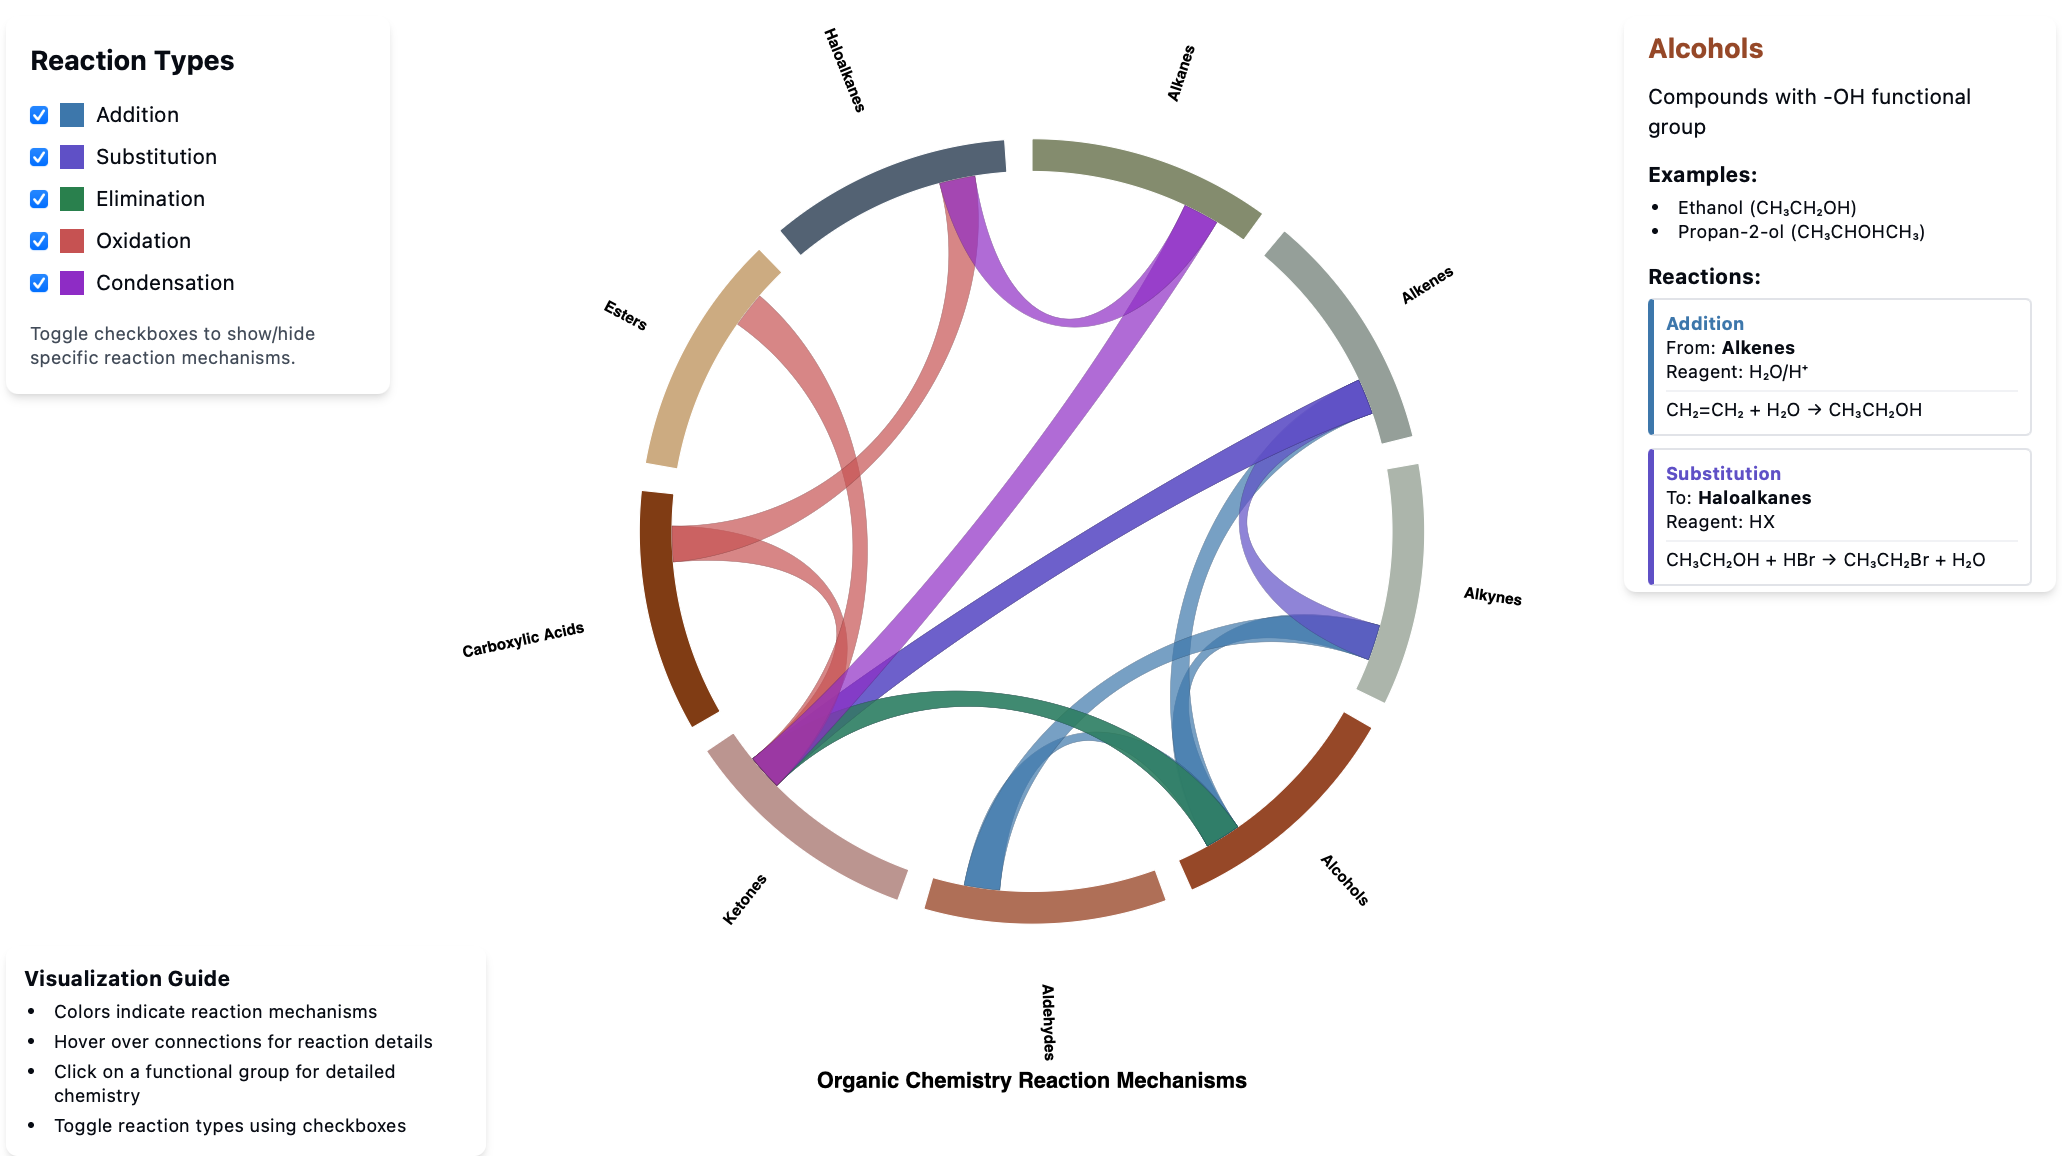
\includegraphics[width=0.7\textwidth]{img/all-organic-chem.png}
        \caption{Overview of Key Functional Group Interconversions}
    \end{figure}
    \vspace{1em}
    \textbf{Challenge Question:} Can we directly convert an Alkane to an Ester using only these reactions? Why/Why not? What intermediates are needed?
    \vspace{1em}
    \textbf{Today's Goal:} Plan more complex syntheses (3+ steps) and communicate them using formal flowcharts.
\end{frame}

\section{Flowchart Conventions}
\begin{frame}{Flowchart Conventions}
    \frametitle{Communicating Synthesis Clearly (CHM\_M7\_SYNTH\_N1)}
    Flowcharts are the standard way to show multi-step syntheses.
    \vspace{1em}
    \textbf{Key Conventions (Worksheet 3):}
    \begin{itemize}
        \item \textbf{Compounds:} In boxes (Use IUPAC Name or Structural Formula).
        \item \textbf{Reactions:} Use arrows $\rightarrow$.
        \item \textbf{Reagents/Conditions:} Write above/below the arrow for THAT step.
        \item \textbf{Layout:} Logical flow (e.g., top-to-bottom).
    \end{itemize}
    \vspace{1em}
    \textbf{Example (Propane $\rightarrow$ Propanone):}
    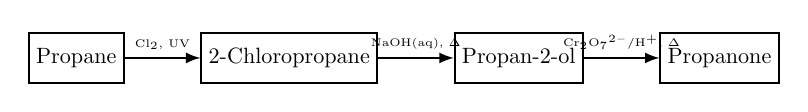
\begin{tikzpicture}[node distance=1.2cm, auto, >=latex, scale=0.8, transform shape,
        compound/.style={rectangle, draw, thick, minimum size=0.8cm, text centered},
        reagent/.style={above, midway, font=\tiny}] % Adjusted font size

        \node [compound] (propane) {Propane};
        \node [compound, right=of propane] (chloro) {2-Chloropropane};
        \node [compound, right=of chloro] (propanol) {Propan-2-ol};
        \node [compound, right=of propanol] (propanone) {Propanone};

        \draw [->, thick] (propane) -- node [reagent] {\ce{Cl2}, UV} (chloro);
        \draw [->, thick] (chloro) -- node [reagent] {NaOH(aq), $\Delta$} (propanol);
        \draw [->, thick] (propanol) -- node [reagent] {\ce{Cr2O7^{2-}/H+}, $\Delta$} (propanone);
    \end{tikzpicture}
\end{frame}

\section{Modelling & Practice}
\begin{frame}{Modelling Complex Synthesis}
    \frametitle{Plan then Draw: Example}
    \textbf{Problem:} Synthesise Propanoic Acid from Propane.
    \vspace{1em}
    \textbf{Teacher Modelling ("Think Aloud"):}
    \begin{enumerate}
        \item \textit{"Start=Alkane, Target=Carboxylic Acid."}
        \item \textit{"Map Check: Alkane $\rightarrow$ Haloalkane $\rightarrow$ Alcohol (Primary needed for Acid) $\rightarrow$ Carboxylic Acid. Path looks viable."} Intermediates: 1-Chloropropane, Propan-1-ol.
        \item \textit{"Translate to Flowchart:"} (Draw step-by-step on board/slide)
            \begin{itemize}
                \item Box 1: Propane (\ce{CH3CH2CH3})
                \item Arrow 1: Reagents \ce{Cl2}, UV Light (Free radical sub gives mix, but targets pathway) $\rightarrow$ Box 2: 1-Chloropropane (\ce{CH3CH2CH2Cl})
                \item Arrow 2: Reagents NaOH(aq), heat (Substitution) $\rightarrow$ Box 3: Propan-1-ol (\ce{CH3CH2CH2OH})
                \item Arrow 3: Reagents \ce{Cr2O7^{2-}/H+}, heat (Oxidation [O]) $\rightarrow$ Box 4: Propanoic Acid (\ce{CH3CH2COOH})
            \end{itemize}
        \item \textit{"Ensure all reagents/conditions and structures/names are correct."}
    \end{enumerate}
\end{frame}

\begin{frame}{Group Synthesis Challenge}
    \frametitle{Design & Build Your Flowchart}
    Work in your groups on the challenge problem from Activity Sheet 3.
    \vspace{1em}
    \textbf{Your Task Recap:}
    \begin{itemize}
        \item Analyse the problem (Start/Target).
        \item Plan your route using the Chord Diagram tool.
        \item Construct a formal, accurate flowchart on your paper/board.
        \item Include all compounds (structures/names) and reagents/conditions.
    \end{itemize}
    \vspace{1em}
    \textbf{Goal:} Create a chemically correct and clearly communicated synthesis plan.
    \vspace{1em}
    \textit{(Teacher circulates, facilitates group work, asks probing questions)}
\end{frame}

\section{Review & Summary}
\begin{frame}{Peer Review & Wrap Up}
    \frametitle{Evaluating Flowcharts}
    Time for Peer Review / Gallery Walk.
    \vspace{1em}
    \begin{itemize}
        \item Display your group's flowchart.
        \item Use the checklist on Activity Sheet 3 to review another group's work.
        \item Focus on: Logical Steps, Correct Chemistry (Structures/Reagents), Clear Conventions.
        \item Provide constructive feedback.
    \end{itemize}
    \vspace{1em}
    \textbf{Final Summary:}
    \begin{itemize}
        \item Synthesis requires integrated knowledge and planning (use the map!).
        \item Flowcharts are the standard way to communicate these plans accurately (CH11/12-7).
    \end{itemize}
    \vspace{1em}
    \textbf{Next Steps:} Complete Exit Ticket. Revise reaction pathways for upcoming assessments.
\end{frame}

\begin{frame}
    \centering
    \textbf{Thank you!}\\ \vspace{1em} Questions?
\end{frame}

\end{document}
